% This LaTeX document needs to be compiled with XeLaTeX.
\documentclass[10pt]{article}
\usepackage[utf8]{inputenc}
\usepackage{ucharclasses}
\usepackage{graphicx}
\usepackage[export]{adjustbox}
\graphicspath{ {./images/} }
\usepackage{amsmath}
\usepackage{amsfonts}
\usepackage{amssymb}
\usepackage[version=4]{mhchem}
\usepackage{stmaryrd}
\usepackage{hyperref}
\hypersetup{colorlinks=true, linkcolor=blue, filecolor=magenta, urlcolor=cyan,}
\urlstyle{same}
\usepackage{multirow}
\usepackage[fallback]{xeCJK}
\usepackage{polyglossia}
\usepackage{fontspec}
\setCJKmainfont{Noto Serif CJK TC}

\setmainlanguage{polish}
\setotherlanguages{thai}
\newfontfamily\thaifont{Noto Serif Thai}
\newfontfamily\lgcfont{CMU Serif}
\setDefaultTransitions{\lgcfont}{}
\setTransitionsFor{Thai}{\thaifont}{\lgcfont}

\title{KOD }

\author{}
\date{}


\begin{document}
\maketitle
IMIĘ I NAZWISKO*\\
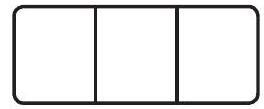
\includegraphics[max width=\textwidth, center]{2024_11_21_4a1915d79134dda0750eg-01}\\
\(\square\)

\begin{itemize}
  \item nieobowiązkowe
\end{itemize}

\section*{PRÓBNY EGZAMIN MATURALNY Z NOWĄ ERĄ MATEMATYKA - POZIOM PODSTAWOWY}
\section*{Instrukcja dla zdającego}
\begin{enumerate}
  \item Sprawdź, czy arkusz egzaminacyjny zawiera 20 stron (zadania 1-33). Ewentualny brak stron zgłoś nauczycielowi nadzorującemu egzamin.
  \item Rozwiązania zadań i odpowiedzi zapisz w miejscu na to przeznaczonym.
  \item Pamiętaj, że pominięcie argumentacji lub istotnych obliczeń w rozwiązaniu zadań otwartych może spowodować, że za to rozwiązanie nie otrzymasz pełnej liczby punktów.
  \item Pisz czytelnie. Używaj długopisu/pióra tylko z czarnym tuszem/atramentem.
  \item Nie używaj korektora, a błędne zapisy wyraźnie przekreśl.
  \item Pamiętaj, że zapisy w brudnopisie nie będą oceniane.
  \item Podczas egzaminu możesz korzystać z zestawu wzorów matematycznych, cyrkla i linijki oraz kalkulatora.
  \item Na tej stronie wpisz swój kod oraz imię i nazwisko.
  \item Odpowiedzi do zadań zamkniętych przenieś na kartę odpowiedzi, zaznaczając je w części karty przeznaczonej dla zdającego.
  \item Nie wpisuj żadnych znaków w części przeznaczonej dla osoby sprawdzającej.
\end{enumerate}

Powodzenia!

Czas pracy:\\
170 minut

Liczba punktów\\
do uzyskania: 50

\section*{ZADANIA ZAMKNIĘTE}
W zadaniach 1-23 wybierz i zaznacz na karcie odpowiedzi poprawną odpowiedź.

\section*{Zadanie 1. (0-1)}
Marek obserwował zwycięski skok Kamila Stocha i oszacował jego długość na 138 m. Oficjalny wynik zawodnika to 132,5 m. Jaki błąd względny popełnił Marek (w zaokrągleniu do części tysięcznych)?\\
A. 0,040\\
B. 0,042\\
C. 0,960\\
D. 5,500

Zadanie 2. (0-1)\\
Liczba \(a\) jest o 20\% mniejsza od liczby b. Jaki procent liczby a stanowi liczba \(b\) ?\\
A. \(20 \%\)\\
B. \(80 \%\)\\
C. \(120 \%\)\\
D. \(125 \%\)

\section*{Zadanie 3. (0-1)}
Iloraz \(\frac{\sqrt{6}-\sqrt{3}}{\sqrt{6}+\sqrt{3}}\) jest równy\\
A. \(3-2 \sqrt{2}\)\\
B. \(\frac{\sqrt{3}}{3}\)\\
C. \(3-6 \sqrt{2}\)\\
D. \(9-2 \sqrt{2}\)

\section*{Zadanie 4. (0-1)}
Zbiorem rozwiązań nierówności \((x-2)^{2} \leqslant 14-(2-x)(x+2)\) jest przedział\\
A. \(\left\langle-\frac{3}{2},+\infty\right)\)\\
B. \(\left(-\frac{3}{2},+\infty\right)\)\\
C. \(\langle-1,3\rangle\)\\
D. \(\left(-\infty,-\frac{3}{2}\right)\)

\section*{Zadanie 5. (0-1)}
Wskaż zdanie nieprawdziwe.\\
A. \(-\sqrt[3]{125}=\sqrt[3]{-125}\)\\
B. \(\sqrt{(-125)^{2}}=-125\)\\
C. \(\sqrt[5]{-64}=-2 \sqrt[5]{2}\)\\
D. \(5^{\frac{7}{3}}=25 \sqrt[3]{5}\)

\section*{Zadanie 6. (0-1)}
Po przesunięciu wykresu funkcji wykładniczej wzdłuż osi \(O y\) układu współrzędnych otrzymano wykres przedstawiony na rysunku. Jest to wykres funkcji\\
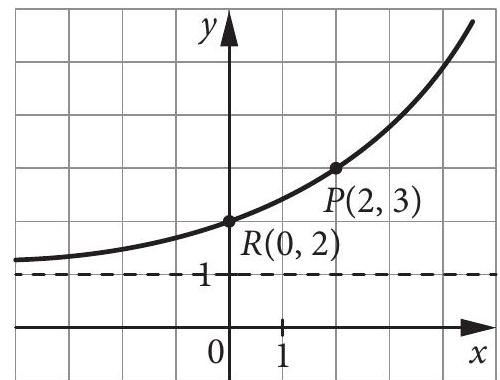
\includegraphics[max width=\textwidth, center]{2024_11_21_4a1915d79134dda0750eg-02}\\
A. \(f(x)=\frac{4}{x}+1\)\\
B. \(f(x)=(\sqrt{2})^{x}+1\)\\
C. \(f(x)=(\sqrt{3})^{\frac{1}{2} x+1}\)\\
D. \(f(x)=(\sqrt{2})^{x-1}\)

Więcej arkuszy znajdziesz na stronie: \href{http://arkusze.pl}{arkusze.pl}\\

\includegraphics[max width=\textwidth, center]{2024_11_21_4a1915d79134dda0750eg-03}

Zadanie 7. (0-1)\\
Liczby \(a\) i \(b\) są dodatnie, \(b \neq 1\) i \(\log _{b} a=4\). Wyrażenie \(\log _{b} \sqrt[3]{a b^{2}}\) przyjmuje wartość\\
A. \(\frac{8}{9}\)\\
B. 2\\
C. \(\frac{14}{3}\)\\
D. 12

\section*{Zadanie 8. (0-1)}
Wykres funkcji liniowej \(f(x)=3 x-2\) odbito symetrycznie względem osi \(O y\). Otrzymano wykres funkcji\\
A. \(g(x)=-3 x+2\)\\
B. \(g(x)=3 x+2\)\\
C. \(g(x)=-3 x-2\)\\
D. \(g(x)=3 x-2\)

\section*{Zadanie 9. (0-1)}
Wskaż oś liczbową, na której przedstawiono zbiór wszystkich wartości \(p\), dla których funkcja liniowa \(f(x)=\left(8-p^{2}\right) x+p\) jest rosnąca.\\
A.\\
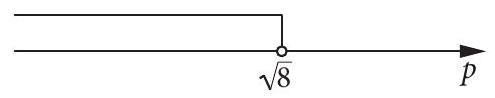
\includegraphics[max width=\textwidth, center]{2024_11_21_4a1915d79134dda0750eg-04(1)}\\
C.\\
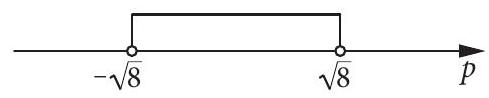
\includegraphics[max width=\textwidth, center]{2024_11_21_4a1915d79134dda0750eg-04(3)}\\
B.\\
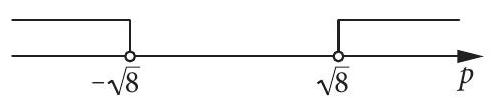
\includegraphics[max width=\textwidth, center]{2024_11_21_4a1915d79134dda0750eg-04(2)}\\
D.\\
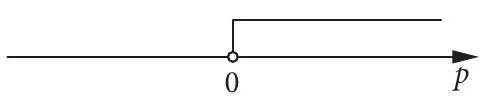
\includegraphics[max width=\textwidth, center]{2024_11_21_4a1915d79134dda0750eg-04}

\section*{Zadanie 10. (0-1)}
Wykres funkcji \(f(x)=-\frac{1}{2}(x-3)^{2}+2\) ma dwa punkty wspólne z prostą o równaniu \(y=m\), jeżeli\\
A. \(m<2\)\\
B. \(m=2\)\\
C. \(m=3\)\\
D. \(m>3\)

Zadanie 11. (0-1)\\
Punkty \(M=(-2,0)\) i \(N=(2,4)\) są wierzchołkami trójkąta równobocznego. Wysokość tego trójkąta jest równa\\
A. \(4 \sqrt{2}\)\\
B. \(2 \sqrt{2}\)\\
C. \(2 \sqrt{6}\)\\
D. \(8 \sqrt{3}\)

Zadanie 12. (0-1)\\
Wzór ogólny ciągu \(\left(a_{n}\right)\) określonego dla wszystkich liczb naturalnych \(n \geqslant 1\) ma postać \(a_{n}=\sqrt{n^{3}} \cdot \sqrt[3]{n} \cdot \sqrt[6]{n}\). Wynika stąd, że\\
A. \(a_{3}=\sqrt[11]{243}\)\\
B. \(a_{3}=9\)\\
C. \(a_{3}=\sqrt[6]{243}\)\\
D. \(a_{3}=2\)

\section*{Zadanie 13. (0-1)}
Dany jest nieskończony ciąg \(\left(a_{n}\right)\), w którym \(a_{1}=4^{10}\), a każdy następny wyraz jest dwukrotnie mniejszy od poprzedniego. Wtedy wyraz \(a_{15}\) jest równy\\
A. 32\\
B. 64\\
C. \(\frac{4^{10}}{15}\)\\
D. \(8^{-4}\)

Więcej arkuszy znajdziesz na stronie: \href{http://arkusze.pl}{arkusze.pl}\\

\includegraphics[max width=\textwidth, center]{2024_11_21_4a1915d79134dda0750eg-05}

\section*{Zadanie 14. (0-1)}
Na rysunku przedstawiono interpretację geometryczną jednego z niżej zapisanych układów równań.\\
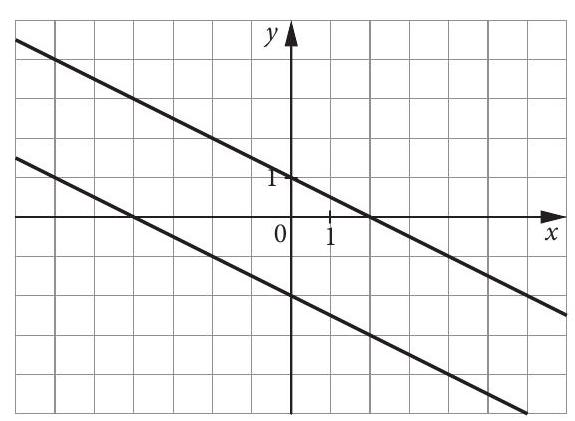
\includegraphics[max width=\textwidth, center]{2024_11_21_4a1915d79134dda0750eg-06}

Wskaż ten układ.\\
A. \(\left\{\begin{array}{l}y=-\frac{1}{2} x-2 \\ y=-\frac{1}{2} x+1\end{array}\right.\)\\
B. \(\left\{\begin{array}{l}y=\frac{1}{2} x-2 \\ y=\frac{1}{2} x+1\end{array}\right.\)\\
C. \(\left\{\begin{array}{l}y=-\frac{1}{2} x+2 \\ y=-\frac{1}{2} x-1\end{array}\right.\)\\
D. \(\left\{\begin{array}{l}y=-2 x-2 \\ y=2 x+1\end{array}\right.\)

Zadanie 15. (0-1)\\
Zależność temperatury w skali Fahrenheita ( \({ }^{\circ} \mathrm{F}\) ) od temperatury w skali Celsjusza ( \({ }^{\circ} \mathrm{C}\) ) wyraża się wzorem: \(f=\frac{9}{5} c+32\), gdzie \(f\) oznacza temperaturę w skali Fahrenheita, a \(c-\mathrm{w}\) skali Celsjusza. 25 maja 2014 r. o godzinie 12 czasu lokalnego temperatura w Warszawie wynosiła \(20^{\circ} \mathrm{C}\), a w Nowym Jorku \(77^{\circ}\) F. O ile stopni temperatura w Nowym Jorku była wyższa od temperatury w Warszawie?\\
A. o \(57^{\circ} \mathrm{F}\)\\
B. \(\quad 25^{\circ} \mathrm{F}\)\\
C. o \(11{ }^{\circ} \mathrm{F}\)\\
D. \(o 9^{\circ} \mathrm{F}\)

\section*{Zadanie 16. (0-1)}
Rzucono równocześnie trzema sześciennymi kostkami do gry. Prawdopodobieństwo, że na wszystkich kostkach wypadła taka sama liczba oczek, jest równe\\
A. \(\frac{1}{6}\)\\
B. \(\frac{1}{6^{2}}\)\\
C. \(\frac{1}{6^{3}}\)\\
D. \(\frac{3}{6^{3}}\)

\section*{Zadanie 17. (0-1)}
W trójkąt równoramienny \(A B C\) o podstawie \(A B\) wpisano okrąg o promieniu 5. Odległość wierzchołka \(C\) od punktu styczności \(S\) okręgu z ramieniem \(B C\) jest równa 12. Wysokość \(C D\) tego trójkąta ma długość\\
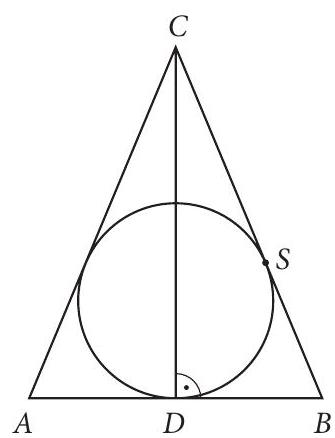
\includegraphics[max width=\textwidth, center]{2024_11_21_4a1915d79134dda0750eg-06(1)}\\
A. 10\\
B. 15\\
C. \(5+\sqrt{119}\)\\
D. 18

Więcej arkuszy znajdziesz na stronie: \href{http://arkusze.pl}{arkusze.pl}\\

\includegraphics[max width=\textwidth, center]{2024_11_21_4a1915d79134dda0750eg-07}

Zadanie 18. (0-1)\\
Wskaż poprawną wartość funkcji trygonometrycznej kąta rozwartego \(\alpha\) (rysunek obok).\\
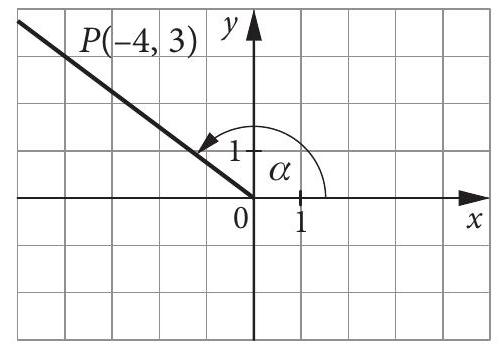
\includegraphics[max width=\textwidth, center]{2024_11_21_4a1915d79134dda0750eg-08(1)}\\
A. \(\cos \alpha=-\frac{4}{5}\)\\
B. \(\cos \alpha=\frac{4}{5}\)\\
C. \(\sin \alpha=\frac{3}{4}\)\\
D. \(\operatorname{tg} \alpha=-\frac{4}{3}\)

\section*{Zadanie 19. (0-1)}
Na trójkącie \(A B C\) opisano okrąg o środku \(S\) i promieniu równym 6. Kąt wpisany \(A C B\) ma miarę \(15^{\circ}\). Pole trójkąta \(A B S\) jest równe\\
A. 9\\
B. \(9 \sqrt{2}\)\\
C. \(9 \sqrt{3}\)\\
D. 18\\
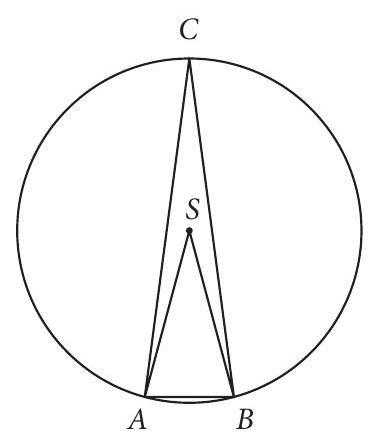
\includegraphics[max width=\textwidth, center]{2024_11_21_4a1915d79134dda0750eg-08}

Zadanie 20. (0-1)\\
Ile jest wszystkich naturalnych liczb trzycyfrowych podzielnych przez 5, w których cyfra dziesiątek jest liczbą pierwszą? (Uwaga: 1 nie jest liczbą pierwszą.)\\
A. 53\\
B. 72\\
C. 90\\
D. 100

Zadanie 21. (0-1)\\
Wszystkie oceny Ani z matematyki to 5, 4, 6, 5, 5 i nieznana ocena \(x\). Średnia arytmetyczna wszystkich ocen Ani jest większa niż ich mediana. Tą oceną może być\\
A. 3\\
B. 4\\
C. 5\\
D. 6

\section*{Zadanie 22. (0-1)}
W graniastosłupie prawidłowym czworokątnym, którego krawędź podstawy ma długość \(a\), pole powierzchni bocznej jest 8 razy większe od pola podstawy. Objętość tego graniastosłupa wynosi\\
A. \(8 a^{3}\)\\
B. \(2 a^{3}\)\\
C. \(\frac{a^{3}}{32}\)\\
D. \(\frac{2}{3} a^{3}\)

\section*{Zadanie 23. (0-1)}
Dany jest stożek, którego tworząca ma długość 4 , a kąt rozwarcia wynosi \(120^{\circ}\). Pole powierzchni bocznej tego stożka jest równe\\
A. \(8 \sqrt{3} \pi\)\\
B. \(4 \pi(2 \sqrt{3}+3)\)\\
C. \(8 \pi\)\\
D. \(\frac{8 \sqrt{3} \pi}{3}\)

Więcej arkuszy znajdziesz na stronie: \href{http://arkusze.pl}{arkusze.pl}\\

\includegraphics[max width=\textwidth, center]{2024_11_21_4a1915d79134dda0750eg-09}

\section*{ZADANIA OTWARTE}
Rozwiązania zadań 24-33 należy zapisać w wyznaczonych miejscach pod treścią zadania.

Zadanie 24. (0-2)\\
Wykres funkcji kwadratowej \(f(x)=\frac{1}{2} x^{2}\) przesunięto o cztery jednostki w prawo i otrzymano wykres funkcji \(g(x)\). Wyznacz zbiór wszystkich argumentów \(x\), dla których funkcja \(g(x)\) przyjmuje wartości większe od 2.

\begin{center}
\begin{tabular}{|c|c|c|c|c|c|c|c|c|c|c|c|c|c|c|c|c|c|c|c|c|c|c|c|c|c|c|c|c|c|}
\hline
 &  &  &  &  &  &  &  &  &  &  &  &  &  &  &  &  &  &  &  &  &  &  &  &  &  &  &  &  &  \\
\hline
 &  &  &  &  &  &  &  &  &  &  &  &  &  &  &  &  &  &  &  &  &  &  &  &  &  &  &  &  &  \\
\hline
 &  &  &  &  &  &  &  &  &  &  &  &  &  &  &  &  &  &  &  &  &  &  &  &  &  &  &  &  &  \\
\hline
 &  &  &  &  &  &  &  &  &  &  &  &  &  &  &  &  &  &  &  &  &  &  &  &  &  &  &  &  &  \\
\hline
 &  &  &  &  &  &  &  &  &  &  &  &  &  &  &  &  &  &  &  &  &  &  &  &  &  &  &  &  &  \\
\hline
 &  &  &  &  &  &  &  &  &  &  &  &  &  &  &  &  &  &  &  &  &  &  &  &  &  &  &  &  &  \\
\hline
 &  &  &  &  &  &  &  &  &  &  &  &  &  &  &  &  &  &  &  &  &  &  &  &  &  &  &  &  &  \\
\hline
 &  &  &  &  &  &  &  &  &  &  &  &  &  &  &  &  &  &  &  &  &  &  &  &  &  &  &  &  &  \\
\hline
 &  &  &  &  &  &  &  &  &  &  &  &  &  &  &  &  &  &  &  &  &  &  &  &  &  &  &  &  &  \\
\hline
 &  &  &  &  &  &  &  &  &  &  &  &  &  &  &  &  &  &  &  &  &  &  &  &  &  &  &  &  &  \\
\hline
 &  &  &  &  &  &  &  &  &  &  &  &  &  &  &  &  &  &  &  &  &  &  &  &  &  &  &  &  &  \\
\hline
 &  &  &  &  &  &  &  &  &  &  &  &  &  &  &  &  &  &  &  &  &  &  &  &  &  &  &  &  &  \\
\hline
 &  &  &  &  &  &  &  &  &  &  &  &  &  &  &  &  &  &  &  &  &  &  &  &  &  &  &  &  &  \\
\hline
 &  &  &  &  &  &  &  &  &  &  &  &  &  &  &  &  &  &  &  &  &  &  &  &  &  &  &  &  &  \\
\hline
 &  &  &  &  &  &  &  &  &  &  &  &  &  &  &  &  &  &  &  &  &  &  &  &  &  &  &  &  &  \\
\hline
 &  &  &  &  &  &  &  &  &  &  &  &  &  &  &  &  &  &  &  &  &  &  &  &  &  &  &  &  &  \\
\hline
 &  &  &  &  &  &  &  &  &  &  &  &  &  &  &  &  &  &  &  &  &  &  &  &  &  &  &  &  &  \\
\hline
 &  &  &  &  &  &  &  &  &  &  &  &  &  &  &  &  &  &  &  &  &  &  &  &  &  &  &  &  &  \\
\hline
 &  &  &  &  &  &  &  &  &  &  &  &  &  &  &  &  &  &  &  &  &  &  &  &  &  &  &  &  &  \\
\hline
 &  &  &  &  &  &  &  &  &  &  &  &  &  &  &  &  &  &  &  &  &  &  &  &  &  &  &  &  &  \\
\hline
 &  &  &  &  &  &  &  &  &  &  &  &  &  &  &  &  &  &  &  &  &  &  &  &  &  &  &  &  &  \\
\hline
 &  &  &  &  &  &  &  &  &  &  &  &  &  &  &  &  &  &  &  &  &  &  &  &  &  &  &  &  &  \\
\hline
 &  &  &  &  &  &  &  &  &  &  &  &  &  &  &  &  &  &  &  &  &  &  &  &  &  &  &  &  &  \\
\hline
 &  &  &  &  &  &  &  &  &  &  &  &  &  &  &  &  &  &  &  &  &  &  &  &  &  &  &  &  &  \\
\hline
 &  &  &  &  &  &  &  &  &  &  &  &  &  &  &  &  &  &  &  &  &  &  &  &  &  &  &  &  &  \\
\hline
 &  &  &  &  &  &  &  &  &  &  &  &  &  &  &  &  &  &  &  &  &  &  &  &  &  &  &  &  &  \\
\hline
 &  &  &  &  &  &  &  &  &  &  &  &  &  &  &  &  &  &  &  &  &  &  &  &  &  &  &  &  &  \\
\hline
 &  &  &  &  &  &  &  &  &  &  &  &  &  &  &  &  &  &  &  &  &  &  &  &  &  &  &  &  &  \\
\hline
 &  &  &  &  &  &  &  &  &  &  &  &  &  &  &  &  &  &  &  &  &  &  &  &  &  &  &  &  &  \\
\hline
 &  &  &  &  &  &  &  &  &  &  &  &  &  &  &  &  &  &  &  &  &  &  &  &  &  &  &  &  &  \\
\hline
 &  &  &  &  &  &  &  &  &  &  &  &  &  &  &  &  &  &  &  &  &  &  &  &  &  &  &  &  &  \\
\hline
 &  &  &  &  &  &  &  &  &  &  &  &  &  &  &  &  &  &  &  &  &  &  &  &  &  &  &  &  &  \\
\hline
 &  &  &  &  &  &  &  &  &  &  &  &  &  &  &  &  &  &  &  &  &  &  &  &  &  &  &  &  &  \\
\hline
 &  &  &  &  &  &  &  &  &  &  &  &  &  &  &  &  &  &  &  &  &  &  &  &  &  &  &  &  &  \\
\hline
 &  &  &  &  &  &  &  &  &  &  &  &  &  &  &  &  &  &  &  &  &  &  &  &  &  &  &  &  &  \\
\hline
 &  &  &  &  &  &  &  &  &  &  &  &  &  &  &  &  &  &  &  &  &  &  &  &  &  &  &  &  &  \\
\hline
 &  &  &  &  &  &  &  &  &  &  &  &  &  &  &  &  &  &  &  &  &  &  &  &  &  &  &  &  &  \\
\hline
\end{tabular}
\end{center}

Odpowiedź:

\section*{Zadanie 25. (0-2)}
Rozwiąż równanie \(\frac{x^{2}-9}{x+3}=1-x\).

Więcej arkuszy znajdziesz na stronie: \href{http://arkusze.pl}{arkusze.pl}\\

\includegraphics[max width=\textwidth, center]{2024_11_21_4a1915d79134dda0750eg-11}

Odpowiedź:

\begin{center}
\begin{tabular}{|c|c|c|c|}
\hline
\multirow{2}{*}{\begin{tabular}{c}
Wypełnia \\
sprawdzający \\
\end{tabular}} & Nr zadania & 24 & 25 \\
\cline { 2 - 4 }
 & Maks. liczba pkt & 2 & 2 \\
\cline { 2 - 4 }
 & Uzyskana liczba pkt &  &  \\
\hline
\end{tabular}
\end{center}

Zadanie 26. (0-2)\\
W pudełku znajduje się 10 piłeczek: 3 białe i 7 czarnych. Z pudełka losujemy kolejno dwie piłeczki bez zwracania. Oblicz prawdopodobieństwo, że obie będą czarne.

Więcej arkuszy znajdziesz na stronie: \href{http://arkusze.pl}{arkusze.pl}\\

\includegraphics[max width=\textwidth, center]{2024_11_21_4a1915d79134dda0750eg-12}

Odpowiedź:

Zadanie 27. (0-2)\\
Oblicz pole kwadratu, gdy dane są współrzędne dwóch jego wierzchołków (-1, 1) i (2, 1). Rozpatrz różne przypadki.

Więcej arkuszy znajdziesz na stronie: \href{http://arkusze.pl}{arkusze.pl}\\

\includegraphics[max width=\textwidth, center]{2024_11_21_4a1915d79134dda0750eg-13}

Odpowiedź:

\begin{center}
\begin{tabular}{|c|c|c|c|}
\hline
\multirow{2}{*}{\begin{tabular}{c}
Wypełnia \\
sprawdzający \\
\end{tabular}} & Nr zadania & 26 & 27 \\
\cline { 2 - 4 }
 & Maks. liczba pkt & 2 & 2 \\
\cline { 2 - 4 }
 & Uzyskana liczba pkt &  &  \\
\hline
\end{tabular}
\end{center}

Zadanie 28. (0-2)\\
Uzasadnij, że funkcja kwadratowa \(f(x)=2 x^{2}-3^{9} x+27^{7}\) nie ma miejsc zerowych.

Więcej arkuszy znajdziesz na stronie: \href{http://arkusze.pl}{arkusze.pl}\\

\includegraphics[max width=\textwidth, center]{2024_11_21_4a1915d79134dda0750eg-14}

\section*{Zadanie 29. (0-2)}
Bartek w czasie wakacji podjął pracę w pizzerii. Pracodawca zaproponował mu następujące warunki płacy: za pierwszy dzień pracy 20 zt , a za każdy następny o \(3 \mathrm{zł}\) więcej niż za poprzedni. Bartek w każdym tygodniu pracuje przez 5 dni. Ile łącznie zarobi po 8 tygodniach pracy?\\

\includegraphics[max width=\textwidth, center]{2024_11_21_4a1915d79134dda0750eg-15}

Odpowiedź:

\begin{center}
\begin{tabular}{|c|c|c|c|}
\hline
\multirow{2}{*}{\begin{tabular}{c}
Wypełnia \\
sprawdzający \\
\end{tabular}} & Nr zadania & 28 & 29 \\
\cline { 2 - 4 }
 & Maks. liczba pkt & 2 & 2 \\
\cline { 2 - 4 }
 & Uzyskana liczba pkt &  &  \\
\hline
\end{tabular}
\end{center}

Zadanie 30. (0-2)\\
W trapezie \(A B C D\), w którym \(A B \| C D\), przedłużono ramiona \(A D\) i \(B C\) tak, aby przecięły się w punkcie \(E\). Wiadomo, że \(|A B|=8 \mathrm{~cm},|C D|=2 \mathrm{~cm}\), a pole powstałego trójkąta \(D C E\) jest równe \(2 \mathrm{~cm}^{2}\). Oblicz pole trapezu \(A B C D\).

Więcej arkuszy znajdziesz na stronie: \href{http://arkusze.pl}{arkusze.pl}\\

\includegraphics[max width=\textwidth, center]{2024_11_21_4a1915d79134dda0750eg-16}

Odpowiedź:

\section*{Zadanie 31. (0-4)}
Janek, który chodzi ze średnią prędkością \(4 \frac{\mathrm{~km}}{\mathrm{~h}}\), a biega ze średnią prędkością \(6 \frac{\mathrm{~km}}{\mathrm{~h}}\), zauważy1, że biegnąc na popołudniowy trening koszykówki, przybywa na miejsce o 4 minuty wcześniej niż idąc normalnym krokiem. Jak daleko od domu Janka znajduje się hala treningowa?

\begin{center}
\begin{tabular}{|c|c|c|c|c|c|c|c|c|c|c|c|c|c|c|c|c|c|c|c|c|c|c|c|c|c|c|c|c|c|c|}
\hline
 &  &  &  &  &  &  &  &  &  &  &  &  &  &  &  &  &  &  &  &  &  &  &  &  &  &  &  &  &  &  \\
\hline
 &  &  &  &  &  &  &  &  &  &  &  &  &  &  &  &  &  &  &  &  &  &  &  &  &  &  &  &  &  &  \\
\hline
 &  &  &  &  &  &  &  &  &  &  &  &  &  &  &  &  &  &  &  &  &  &  &  &  &  &  &  &  &  &  \\
\hline
 &  &  &  &  &  &  &  &  &  &  &  &  &  &  &  &  &  &  &  &  &  &  &  &  &  &  &  &  &  &  \\
\hline
 &  &  &  &  &  &  &  &  &  &  &  &  &  &  &  &  &  &  &  &  &  &  &  &  &  &  &  &  &  &  \\
\hline
 &  &  &  &  &  &  &  &  &  &  &  &  &  &  &  &  &  &  &  &  &  &  &  &  &  &  &  &  &  &  \\
\hline
 &  &  &  &  &  &  &  &  &  &  &  &  &  &  &  &  &  &  &  &  &  &  &  &  &  &  &  &  &  &  \\
\hline
 &  &  &  &  &  &  &  &  &  &  &  &  &  &  &  &  &  &  &  &  &  &  &  &  &  &  &  &  &  &  \\
\hline
 &  &  &  &  &  &  &  &  &  &  &  &  &  &  &  &  &  &  &  &  &  &  &  &  &  &  &  &  &  &  \\
\hline
 &  &  &  &  &  &  &  &  &  &  &  &  &  &  &  &  &  &  &  &  &  &  &  &  &  &  &  &  &  &  \\
\hline
 &  &  &  &  &  &  &  &  &  &  &  &  &  &  &  &  &  &  &  &  &  &  &  &  &  &  &  &  &  &  \\
\hline
 &  &  &  &  &  &  &  &  &  &  &  &  &  &  &  &  &  &  &  &  &  &  &  &  &  &  &  &  &  &  \\
\hline
\( \underset{\sim}{*} \) &  &  &  &  &  &  &  &  &  &  &  &  &  &  &  &  &  &  &  &  &  &  &  &  &  &  &  &  &  &  \\
\hline
I &  &  &  &  &  &  &  &  &  &  &  &  &  &  &  &  &  &  &  &  &  &  &  &  &  &  &  &  &  &  \\
\hline
龸 &  &  &  &  &  &  &  &  &  &  &  &  &  &  &  &  &  &  &  &  &  &  &  &  &  &  &  &  &  &  \\
\hline
的 &  &  &  &  &  &  &  &  &  &  &  &  &  &  &  &  &  &  &  &  &  &  &  &  &  &  &  &  &  &  \\
\hline
枵 &  &  &  &  &  &  &  &  &  &  &  &  &  &  &  &  &  &  &  &  &  &  &  &  &  &  &  &  &  &  \\
\hline
臬 &  &  &  &  &  &  &  &  &  &  &  &  &  &  &  &  &  &  &  &  &  &  &  &  &  &  &  &  &  &  \\
\hline
N &  &  &  &  &  &  &  &  &  &  &  &  &  &  &  &  &  &  &  &  &  &  &  &  &  &  &  &  &  &  \\
\hline
N &  &  &  &  &  &  &  &  &  &  &  &  &  &  &  &  &  &  &  &  &  &  &  &  &  &  &  &  &  &  \\
\hline
- &  &  &  &  &  &  &  &  &  &  &  &  &  &  &  &  &  &  &  &  &  &  &  &  &  &  &  &  &  &  \\
\hline
\( \begin{aligned} & \underset{N}{N} \end{aligned} \) &  &  &  &  &  &  &  &  &  &  &  &  &  &  &  &  &  &  &  &  &  &  &  &  &  &  &  &  &  &  \\
\hline
到 &  &  &  & 
\includegraphics[max width=\textwidth]{2024_11_21_4a1915d79134dda0750eg-17}
 &  &  &  &  &  &  &  &  &  &  &  &  &  &  &  &  &  &  &  &  &  &  &  &  &  &  \\
\hline
สี &  &  &  &  &  &  &  &  &  &  &  &  &  &  &  &  &  &  &  &  &  &  &  &  &  &  &  &  &  &  \\
\hline
到 &  &  &  &  &  &  &  &  &  &  &  &  &  &  &  &  &  &  &  &  &  &  &  &  &  &  &  &  &  &  \\
\hline
 &  &  &  &  &  &  &  &  &  &  &  &  &  &  &  &  &  &  &  &  &  &  &  &  &  &  &  &  &  &  \\
\hline
 &  &  &  &  &  &  &  &  &  &  &  &  &  &  &  &  &  &  &  &  &  &  &  &  &  &  &  &  &  &  \\
\hline
 &  &  &  &  &  &  &  &  &  &  &  &  &  &  &  &  &  &  &  &  &  &  &  &  &  &  &  &  &  &  \\
\hline
 &  &  &  &  &  &  &  &  &  &  &  &  &  &  &  &  &  &  &  &  &  &  &  &  &  &  &  &  &  &  \\
\hline
 & - &  &  &  &  &  &  &  &  &  &  &  &  &  &  &  &  &  &  &  &  &  &  &  &  &  &  &  &  &  \\
\hline
 & | &  &  &  &  &  &  &  &  &  &  &  &  &  &  &  &  &  &  &  &  &  &  &  &  &  &  &  &  &  \\
\hline
 &  &  &  &  &  &  &  &  &  &  &  &  &  &  &  &  &  &  &  &  &  &  &  &  &  &  &  &  &  &  \\
\hline
 &  &  &  &  &  &  &  &  &  &  &  &  &  &  &  &  &  &  &  &  &  &  &  &  &  &  &  &  &  &  \\
\hline
 &  &  &  &  &  &  &  &  &  &  &  &  &  &  &  &  &  &  &  &  &  &  &  &  &  &  &  &  &  &  \\
\hline
 &  &  &  &  &  &  &  &  &  &  &  &  &  &  &  &  &  &  &  &  &  &  &  &  &  &  &  &  &  &  \\
\hline
 &  &  &  &  &  &  &  &  &  &  &  &  &  &  &  &  &  &  &  &  &  &  &  &  &  &  &  &  &  &  \\
\hline
\end{tabular}
\end{center}

Odpowiedź:

\begin{center}
\begin{tabular}{|c|c|c|c|}
\hline
\multirow{2}{*}{\begin{tabular}{c}
Wypełnia \\
sprawdzający \\
\end{tabular}} & Nr zadania & 30 & 31 \\
\cline { 2 - 4 }
 & Maks. liczba pkt & 2 & 4 \\
\cline { 2 - 4 }
 & Uzyskana liczba pkt &  &  \\
\hline
\end{tabular}
\end{center}

Zadanie 32. (0-5)\\
Punkty \(A=(-2,-4), B=(8,1), C=(4,4)\) są kolejnymi wierzchołkami trapezu równoramiennego \(A B C D\) (niebędącego równoległobokiem) o podstawach \(A B\) oraz \(C D\).\\
a) Wyznacz równanie prostej, która jest osią symetrii tego trapezu.\\
b) Oblicz współrzędne punktu będącego środkiem podstawy \(C D\).\\

\includegraphics[max width=\textwidth, center]{2024_11_21_4a1915d79134dda0750eg-18}

\section*{Zadanie 33. (0-4)}
W czworościanie foremnym, którego krawędź ma długość \(a\), kąt \(\alpha\) jest kątem nachylenia krawędzi bocznej do płaszczyzny podstawy. Oblicz wartość wyrażenia \(\cos ^{2}\left(90^{\circ}-\alpha\right)-\cos ^{2} \alpha\).\\
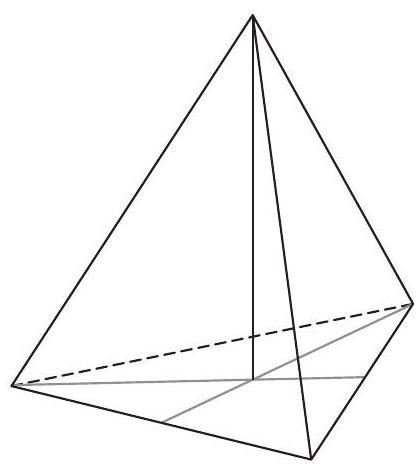
\includegraphics[max width=\textwidth, center]{2024_11_21_4a1915d79134dda0750eg-19}

\begin{center}
\begin{tabular}{|c|c|c|c|c|c|c|c|c|c|c|c|c|c|c|c|c|c|c|c|c|c|c|c|c|c|c|c|c|c|}
\hline
 &  &  &  &  &  &  &  &  &  &  &  &  &  &  &  &  &  &  &  &  &  &  &  &  &  &  &  &  &  \\
\hline
 &  &  &  &  &  &  &  &  &  &  &  &  &  &  &  &  &  &  &  &  &  &  &  &  &  &  &  &  &  \\
\hline
 &  &  &  &  &  &  &  &  &  &  &  &  &  &  &  &  &  &  &  &  &  &  &  &  &  &  &  &  &  \\
\hline
 &  &  &  &  &  &  &  &  &  &  &  &  &  &  &  &  &  &  &  &  &  &  &  &  &  &  &  &  &  \\
\hline
 &  &  &  &  &  &  &  &  &  &  &  &  &  &  &  &  &  &  &  &  &  &  &  &  &  &  &  &  &  \\
\hline
 &  &  &  &  &  &  &  &  &  &  &  &  &  &  &  &  &  &  &  &  &  &  &  &  &  &  &  &  &  \\
\hline
 &  &  &  &  &  &  &  &  &  &  &  &  &  &  &  &  &  &  &  &  &  &  &  &  &  &  &  &  &  \\
\hline
 &  &  &  &  &  &  &  &  &  &  &  &  &  &  &  &  &  &  &  &  &  &  &  &  &  &  &  &  &  \\
\hline
 &  &  &  &  &  &  &  &  &  &  &  &  &  &  &  &  &  &  &  &  &  &  &  &  &  &  &  &  &  \\
\hline
 &  &  &  &  &  &  &  &  &  &  &  &  &  &  &  &  &  &  &  &  &  &  &  &  &  &  &  &  &  \\
\hline
 &  &  &  &  &  &  &  &  &  &  &  &  &  &  &  &  &  &  &  &  &  &  &  &  &  &  &  &  &  \\
\hline
 &  &  &  &  &  &  &  &  &  &  &  &  &  &  &  &  &  &  &  &  &  &  &  &  &  &  &  &  &  \\
\hline
 &  &  &  &  &  &  &  &  &  &  &  &  &  &  &  &  &  &  &  &  &  &  &  &  &  &  &  &  &  \\
\hline
 &  &  &  &  &  &  &  &  &  &  &  &  &  &  &  &  &  &  &  &  &  &  &  &  &  &  &  &  &  \\
\hline
 &  &  &  &  &  &  &  &  &  &  &  &  &  &  &  &  &  &  &  &  &  &  &  &  &  &  &  &  &  \\
\hline
 &  &  &  &  &  &  &  &  &  &  &  &  &  &  &  &  &  &  &  &  &  &  &  &  &  &  &  &  &  \\
\hline
 &  &  &  &  &  &  &  &  &  &  &  &  &  &  &  &  &  &  &  &  &  &  &  &  &  &  &  &  &  \\
\hline
 &  &  &  &  &  &  &  &  &  &  &  &  &  &  &  &  &  &  &  &  &  &  &  &  &  &  &  &  &  \\
\hline
 &  &  &  &  &  &  &  &  &  &  &  &  &  &  &  &  &  &  &  &  &  &  &  &  &  &  &  &  &  \\
\hline
 &  &  &  &  &  &  &  &  &  &  &  &  &  &  &  &  &  &  &  &  &  &  &  &  &  &  &  &  &  \\
\hline
 &  &  &  &  &  &  &  &  &  &  &  &  &  &  &  &  &  &  &  &  &  &  &  &  &  &  &  &  &  \\
\hline
 &  &  &  &  &  &  &  &  &  &  &  &  &  &  &  &  &  &  &  &  &  &  &  &  &  &  &  &  &  \\
\hline
 &  &  &  &  &  &  &  &  &  &  &  &  &  &  &  &  &  &  &  &  &  &  &  &  &  &  &  &  &  \\
\hline
 &  &  &  &  &  &  &  &  &  &  &  &  &  &  &  &  &  &  &  &  &  &  &  &  &  &  &  &  &  \\
\hline
 &  &  &  &  &  &  &  &  &  &  &  &  &  &  &  &  &  &  &  &  &  &  &  &  &  &  &  &  &  \\
\hline
 &  &  &  &  &  &  &  &  &  &  &  &  &  &  &  &  &  &  &  &  &  &  &  &  &  &  &  &  &  \\
\hline
 &  &  &  &  &  &  &  &  &  &  &  &  &  &  &  &  &  &  &  &  &  &  &  &  &  &  &  &  &  \\
\hline
 &  &  &  &  &  &  &  &  &  &  &  &  &  &  &  &  &  &  &  &  &  &  &  &  &  &  &  &  &  \\
\hline
\end{tabular}
\end{center}

Odpowiedź:

\begin{center}
\begin{tabular}{|c|c|c|c|}
\hline
\multirow{3}{*}{\begin{tabular}{c}
Wypełnia \\
sprawdzający \\
\end{tabular}} & Nr zadania & 32 & 33 \\
\cline { 2 - 4 }
 & Maks. liczba pkt & 5 & 4 \\
\cline { 2 - 4 }
 & Uzyskana liczba pkt &  &  \\
\hline
\end{tabular}
\end{center}

Więcej arkuszy znajdziesz na stronie: \href{http://arkusze.pl}{arkusze.pl} \begin{tabular}{|l|l|l|l|l|l|l|l|l|l|l|l|l|l|l|l|l|l|l|l|l|l|l|l|l|l|l|l|l|l|}
\hline
\end{tabular}


\includegraphics[max width=\textwidth, center]{2024_11_21_4a1915d79134dda0750eg-20}\\
\(\qquad\)\\
\(\qquad\)\\
\(\qquad\)\\
\(\qquad\)\\
\(\qquad\)\\
\(\qquad\)\\
\(\qquad\)\\
\(\qquad\)\\
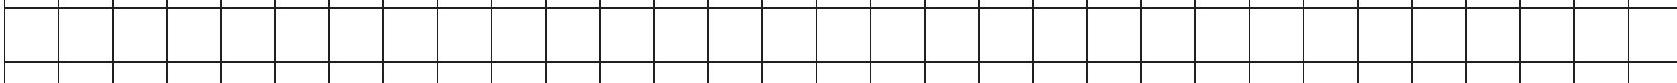
\includegraphics[max width=\textwidth, center]{2024_11_21_4a1915d79134dda0750eg-20(1)}\\
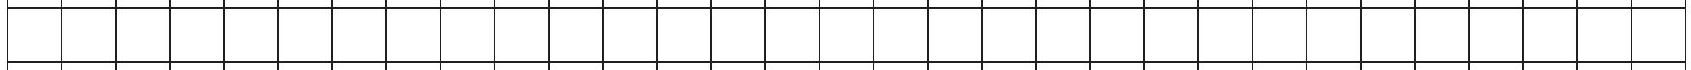
\includegraphics[max width=\textwidth, center]{2024_11_21_4a1915d79134dda0750eg-20(2)}\\

\includegraphics[max width=\textwidth, center]{2024_11_21_4a1915d79134dda0750eg-21}

\begin{itemize}
  \item nieobowiązkowe
\end{itemize}

KARTA ODPOWIEDZI\\
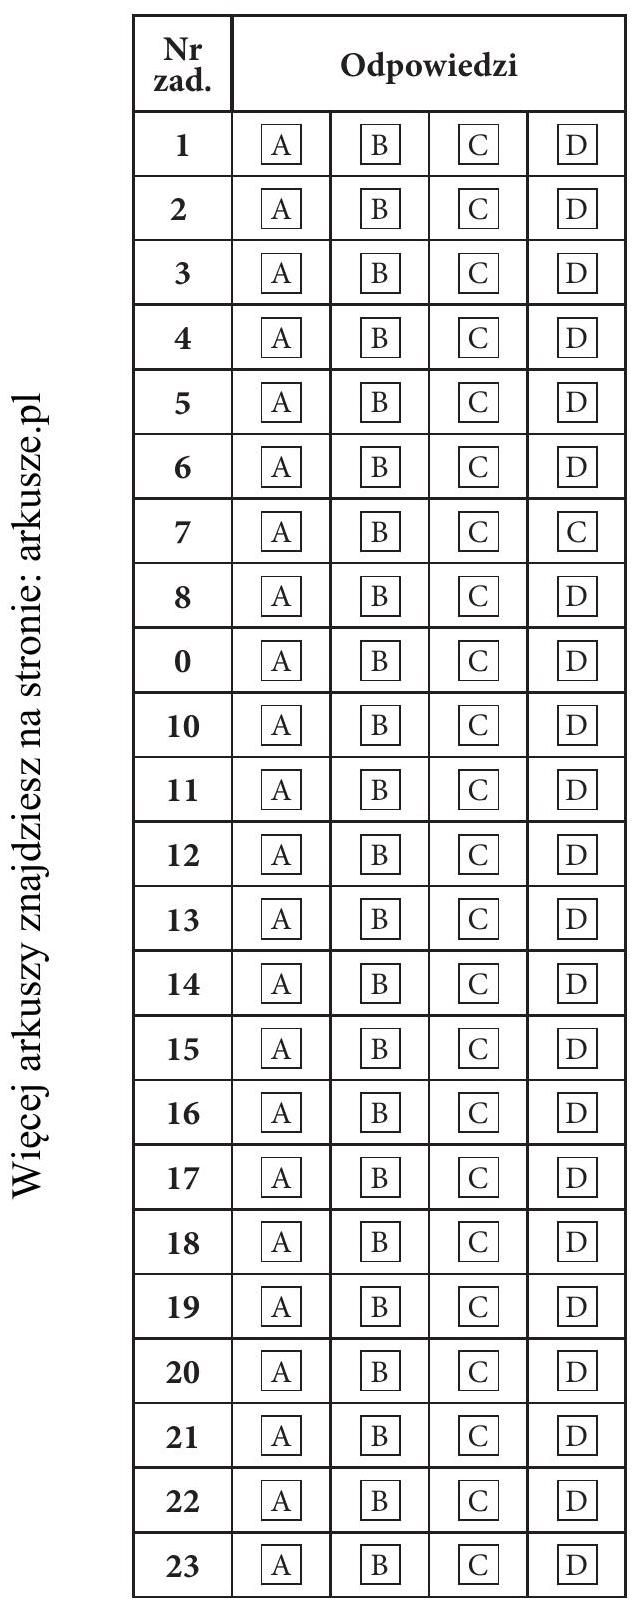
\includegraphics[max width=\textwidth, center]{2024_11_21_4a1915d79134dda0750eg-21(1)}

WYPEŁNIA SPRAWDZAJĄCY

\begin{center}
\begin{tabular}{|c|c|c|c|c|c|c|}
\hline
\multirow{2}{*}{\begin{tabular}{c}
Nr \\
zad. \\
\end{tabular}} & \multicolumn{6}{|c|}{Punkty} \\
\hline
 & \(\mathbf{0}\) & \(\mathbf{1}\) & \(\mathbf{2}\) & \(\mathbf{3}\) & \(\mathbf{4}\) & \(\mathbf{5}\) \\
\hline
\(\mathbf{2 4}\) & \(\square\) & \(\square\) & \(\square\) &  &  &  \\
\hline
\(\mathbf{2 5}\) & \(\square\) & \(\square\) & \(\square\) &  &  &  \\
\hline
\(\mathbf{2 6}\) & \(\square\) & \(\square\) & \(\square\) &  &  &  \\
\hline
\(\mathbf{2 7}\) & \(\square\) & \(\square\) & \(\square\) &  &  &  \\
\hline
\(\mathbf{2 8}\) & \(\square\) & \(\square\) & \(\square\) &  &  &  \\
\hline
\(\mathbf{2 9}\) & \(\square\) & \(\square\) & \(\square\) &  &  &  \\
\hline
\(\mathbf{3 0}\) & \(\square\) & \(\square\) & \(\square\) &  &  &  \\
\hline
\(\mathbf{3 1}\) & \(\square\) & \(\square\) & \(\square\) & \(\square\) & \(\square\) &  \\
\hline
\(\mathbf{3 2}\) & \(\square\) & \(\square\) & \(\square\) & \(\square\) & \(\square\) & \(\square\) \\
\hline
\(\mathbf{3 3}\) & \(\square\) & \(\square\) & \(\square\) & \(\square\) & \(\square\) &  \\
\hline
\end{tabular}
\end{center}


\end{document}